\documentclass{standalone}

\usepackage{tikz}
\usetikzlibrary{decorations.markings}

\begin{document}

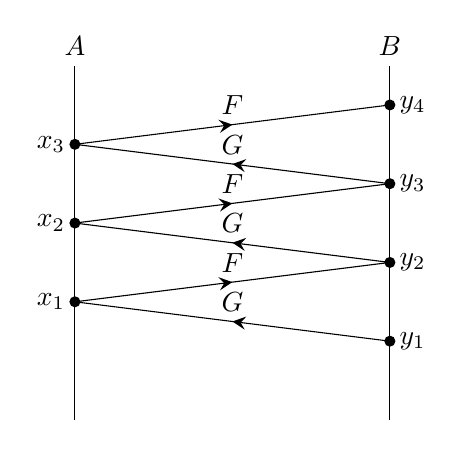
\begin{tikzpicture}[decoration={markings,
    mark=at position 0.5 with {
      \arrow[>=stealth, scale=1.5]{>};
    }}
  ]
  
   % Define coordinates
  \coordinate (A) at (0,0);
  \coordinate (B) at (4,0);
  \coordinate (x1) at (0,1.5);
  \coordinate (x2) at (0,2.5);
  \coordinate (x3) at (0,3.5);
  \coordinate (y1) at (4,1);
  \coordinate (y2) at (4,2);
  \coordinate (y3) at (4,3);
  \coordinate (y4) at (4,4);

  % Draw lines and nodes 
  % Using relative coordinates: ++
  \draw (A) -- ++(0,4.5) node[above] {$A$}; % Vertical line A
  \draw (B) -- ++(0,4.5) node[above] {$B$}; % Vertical line B

  \foreach \i in {1,2,3} {
    \draw[postaction={decorate}] (y\i) --  (x\i) node[midway,above] {$G$};
    \draw[postaction={decorate}] (x\i) -- (y\the\numexpr\i+1\relax) node[midway,above] {$F$};
    \fill (x\i) circle (2pt) node[left] {$x_\i$};
    \fill (y\i) circle (2pt) node[right] {$y_\i$};
  }
  \fill (y4) circle (2pt) node[right] {$y_4$};

\end{tikzpicture}

\end{document}